\documentclass[10pt,a4paper]{article}
\usepackage[utf8]{inputenc}
\usepackage{amsmath}
\usepackage{amsfonts}
\usepackage{graphicx}
\usepackage{amssymb}
\usepackage[numbers,sort&compress]{natbib}
\usepackage[left=2cm,right=2cm,top=1.1cm,bottom=2cm]{geometry}
\usepackage[spanish]{babel}
\usepackage{url}
\usepackage{caption}
\author{Orlando Lázaro Ruiloba Torres\hspace{.4cm}5270}
\title{Tarea 2 Optimización de Flujo en Redes}
\date{\today}

\usepackage{listings}
\usepackage{color}

\definecolor{dkgreen}{rgb}{0,0.6,0}
\definecolor{gray}{rgb}{0.5,0.5,0.5}
\definecolor{mauve}{rgb}{0.58,0,0.82}

\lstset{
	frame=tb,
	language=Python,
	aboveskip=3mm,
	belowskip=3mm,
	showstringspaces=false,
	columns=flexible,
	basicstyle={\small\ttfamily},
	numbers=left,
	numberstyle=\tiny\color{black},
	keywordstyle=\color{blue},
	commentstyle=\color{dkgreen},
	stringstyle=\color{mauve},
	breaklines=true,
	breakatwhitespace=true,
	tabsize=3
}

\begin{document}
\maketitle

\section{Algoritmo de acomodo bipartito}

El diseño de este algoritmo se crea colocando primero los vértices en dos filas, de acuerdo con sus tipos. Luego, las posiciones dentro de las filas se optimizan para minimizar los cruces de arcos, utilizando el algoritmo de Sugiyama \cite{b1}. Este algoritmo de acomodo actualmente solo funciona en dos dimensiones \cite{b2}.\vspace{.4cm}

El código en python se muestra a continuación:

\lstinputlisting[language=Python]{grafo_simple_dirigido_aciclico.py}

\begin{center}

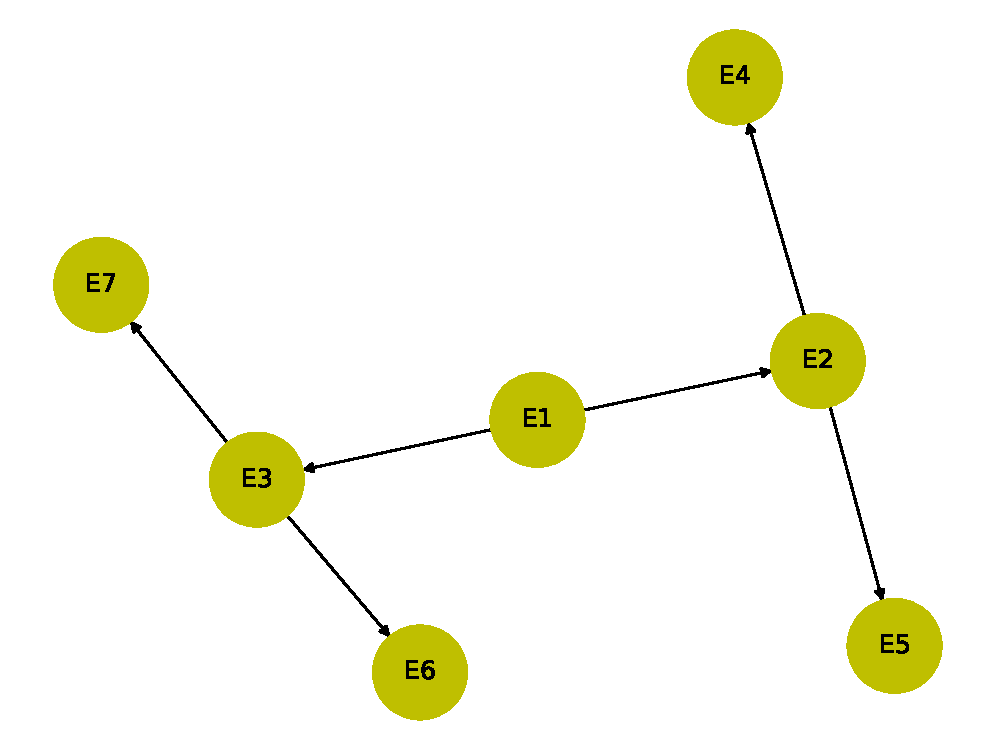
\includegraphics[scale=0.4]{GDA}
\captionof{figure}{Algoritmo bipartito en grafo dirigido acíclico}

\end{center}

\section{Algoritmo de acomodo circular}

Es un algoritmo de diseño que permite colocar los vértices en topologías de anillo y estrella interconectados. Produce diseños que enfatizan las estructuras de grupo y árbol dentro de una red. Crea particiones de nodo mediante el análisis de la estructura de conectividad de la red, y organiza las particiones como círculos separados. Los círculos en sí están dispuestos en forma de árbol radial \cite{c}.\newpage

El código en python es:
 
\lstinputlisting[language=Python]{multigrafo_no_dirigido_ciclico.py}

\begin{center}

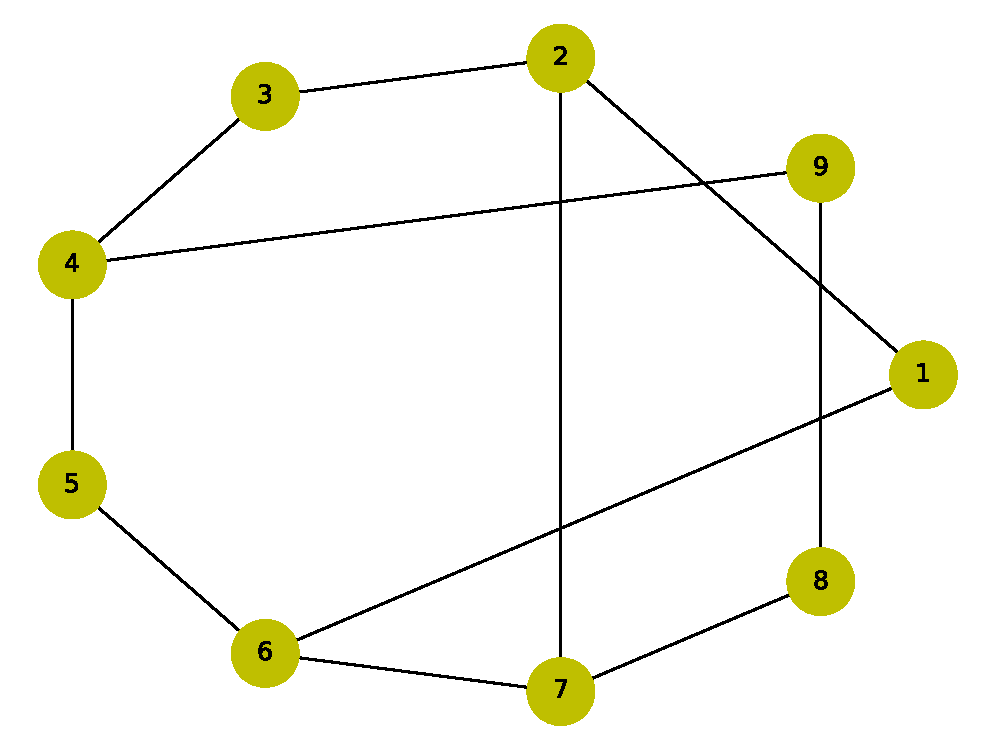
\includegraphics[scale=0.4]{MNDC}
\captionof{figure}{Algoritmo circular en multigrafo no dirigido cíclico}

\end{center}

\section{Algoritmo de acomodo kamada kawai}

Este algoritmo de acomodo se basa en la idea de usar solo fuerzas de resorte entre todos los pares de vértices, el criterio estético que considera es que la distancia entre los vértices debe ser igual a la distancia teórica. Mantiene implícitamente los dos criterios anteriores \cite{d}.\newpage

El código en python se muestra a continuación:

\lstinputlisting[language=Python]{grafo_simple_no_dirigido_reflexivo.py}

\begin{center}

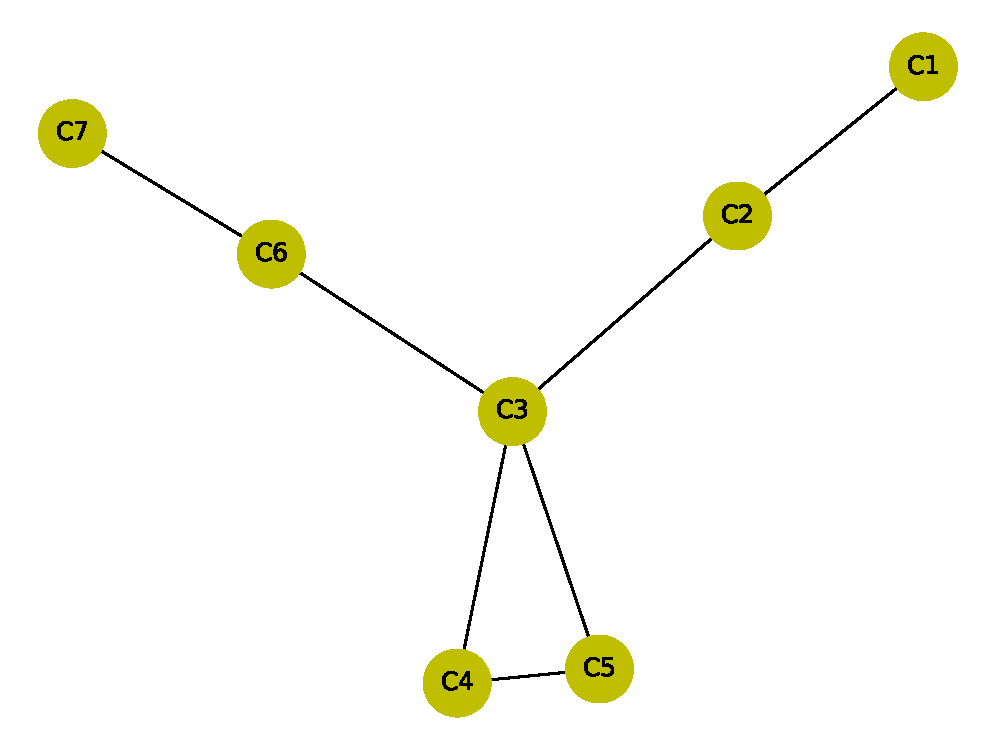
\includegraphics[scale=0.4]{GNDR}
\captionof{figure}{Algoritmo kamada kawai en grafo simple no dirigido reflexivo}

\end{center}

\section{Algoritmo de acomodo aleatorio}

Es un algoritmo que posiciona los vértices uniformemente al azar en el cuadrado unitario. Para cada vértice se genera una posición, al elegir cada una de las coordenadas tenues de la forma mencionada anteriormente en el intervalo [0.0, 1.0] \cite{e}.\vspace{.4cm}

El código en pyhton es el siguiente:

\lstinputlisting[language=Python]{grafo_simple_no_dirigido_ciclico.py}

\begin{center}

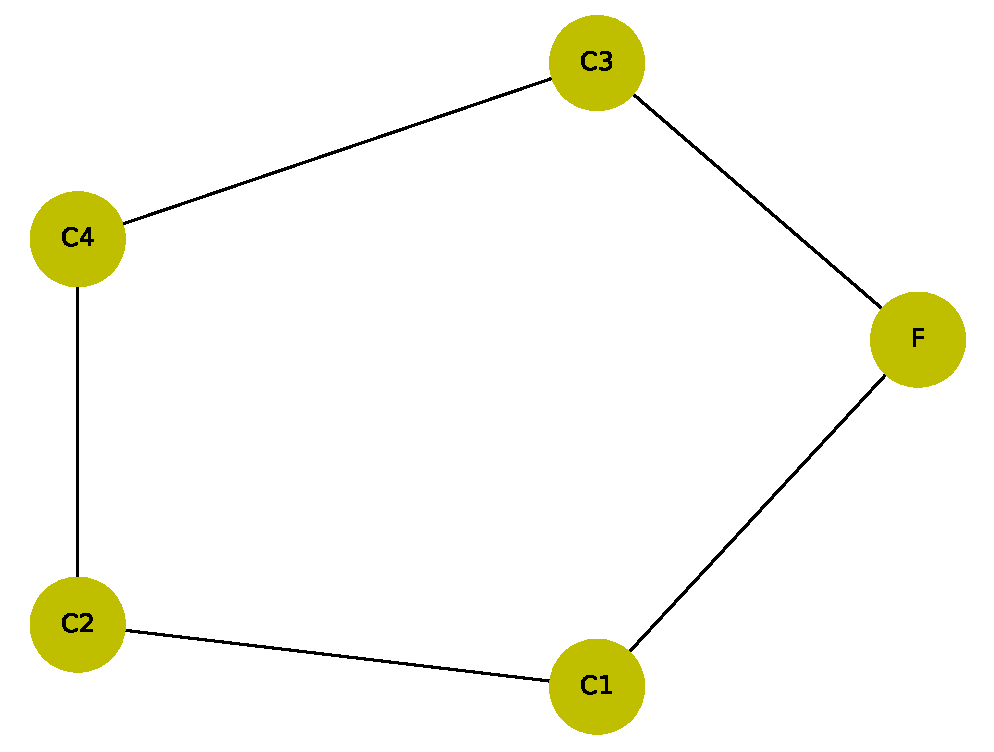
\includegraphics[scale=0.4]{GNDC}
\captionof{figure}{Algoritmo aleatorio en grafo no dirigido cíclico}

\end{center}


\section{Algoritmo de acomodo espectral}

El código en python se muestra a continuación:

\lstinputlisting[language=Python]{multigrafo_no_dirigido_reflexivo.py}

\begin{center}

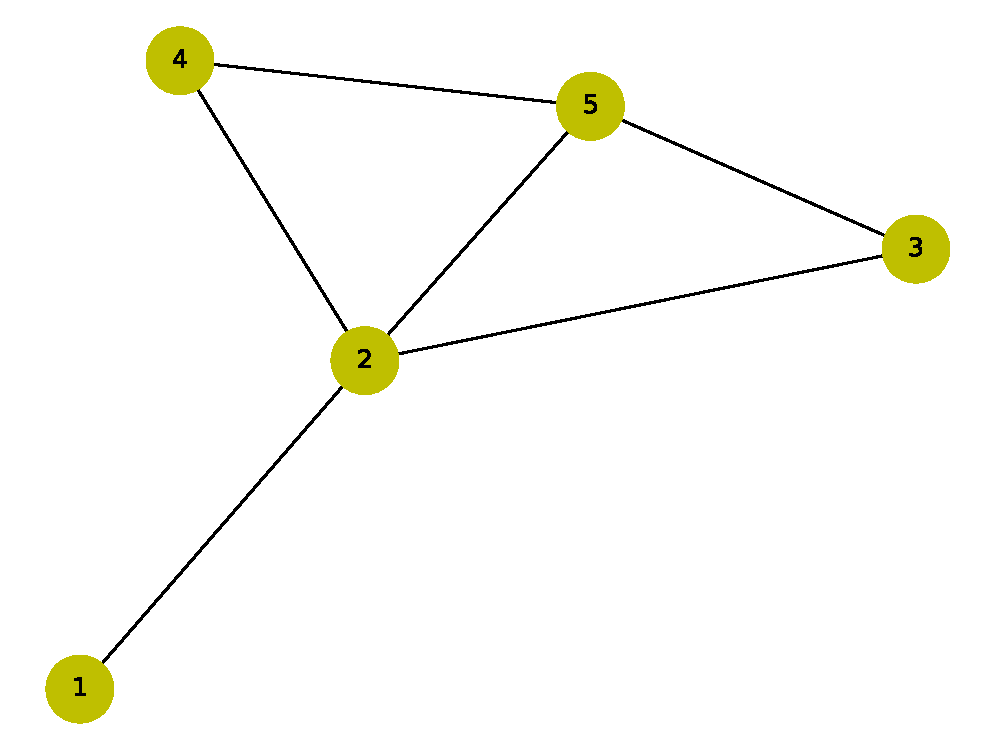
\includegraphics[scale=0.4]{MNDR}
\captionof{figure}{Algoritmo espectral en multigrafo no dirigido reflexivo}

\end{center}

\section{Algoritmo de acomodo shell}

Este algoritmo de acomodo es interesante, ya que le permite al diseñador seleccionar subgrupos de nodos para posicionarlos en círculos concéntricos, en este sentido es menos automático que otros diseños, pero tiene la ventaja crítica de que se puede usar para resaltar características específicas de la red \cite{g}.\newpage

El código en python es:

\lstinputlisting[language=Python]{grafo_simple_dirigido_reflexivo.py}

\begin{center}

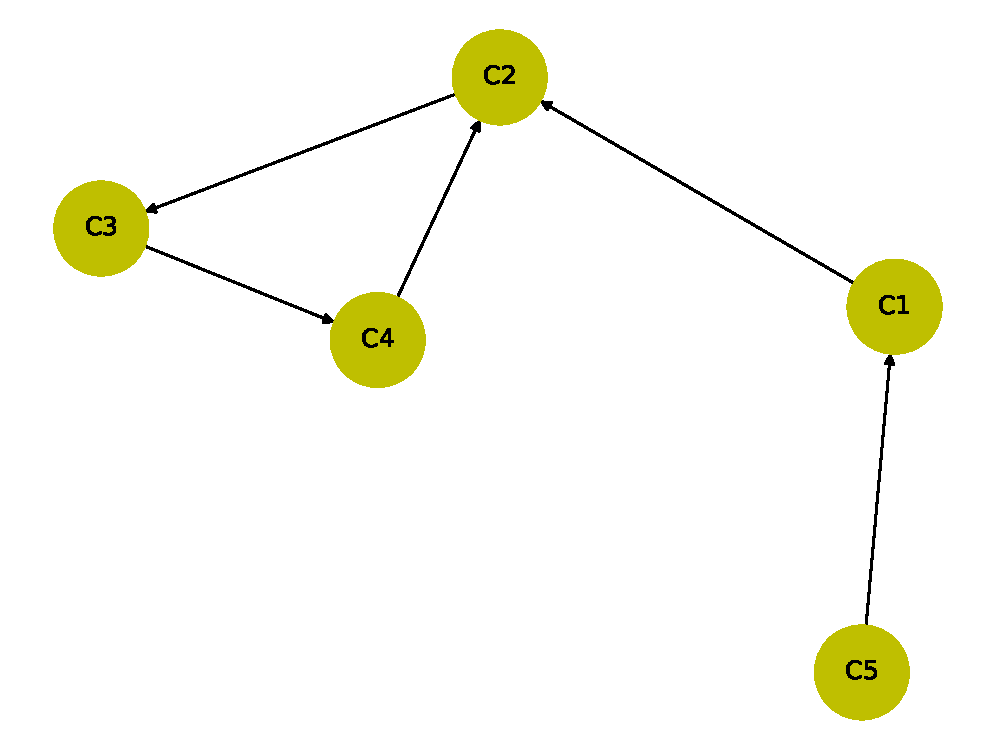
\includegraphics[scale=0.4]{GDR}
\captionof{figure}{Algoritmo shell en grafo dirigido reflexivo}

\end{center}

\section{Algoritmo de acomodo resorte}

En este caso el algoritmo posiciona los nodos basándose en el algoritmo de fuerza dirigida de Fruchterman-Reingold \cite{h}. Cada elemento se trata como una partícula con una carga eléctrica similar que repele otros elementos. Los conectores actúan como resortes que vuelven a unir los elementos conectados. El algoritmo es bueno para resaltar grupos de objetos relacionados e identificar simetría en el grafo \cite{i}.\vspace{.4cm}

El código en python se muestra a continuación:

\lstinputlisting[language=Python]{grafo_simple_no_dirigido_aciclico.py}

\begin{center}

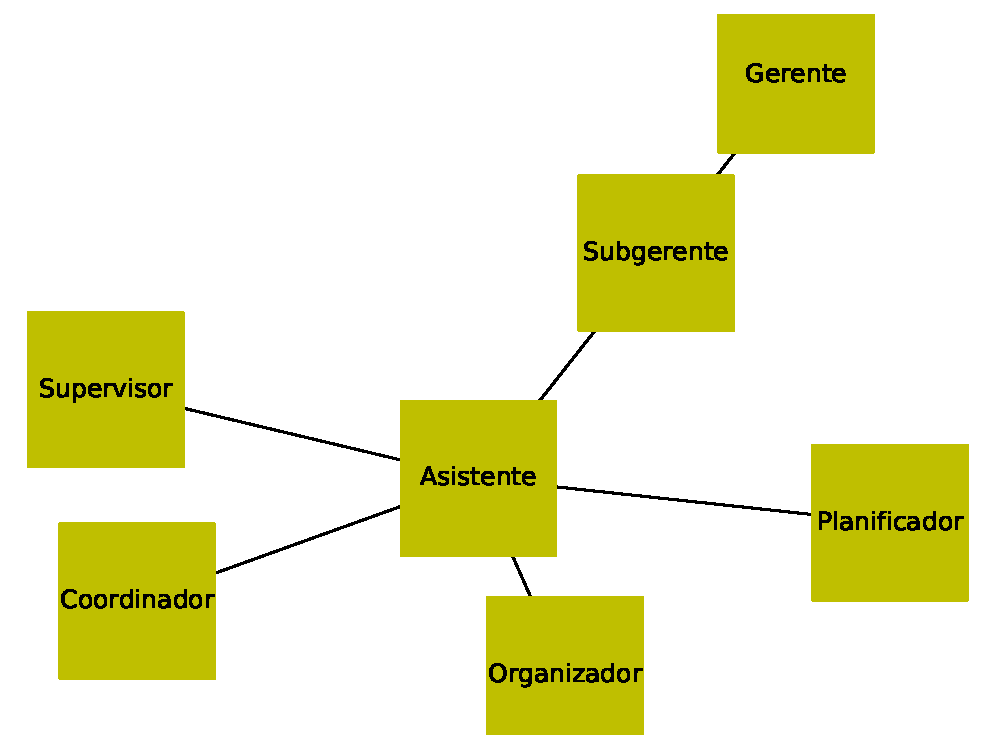
\includegraphics[scale=0.4]{GNDA}
\captionof{figure}{Algoritmo resorte en grafo no dirigido acíclico}

\end{center}


\section{Algoritmo de acomodo espectral}

Este algoritmo posiciona los nodos utilizando los vectores propios del grafo Laplaciano, el diseño muestra posibles agrupaciones de nodos que son una aproximación de la relación de corte \cite{j}.\vspace{.4cm}

El código en python es el siguiente:

\lstinputlisting[language=Python]{multigrafo_dirigido_ciclico.py}

\begin{center}

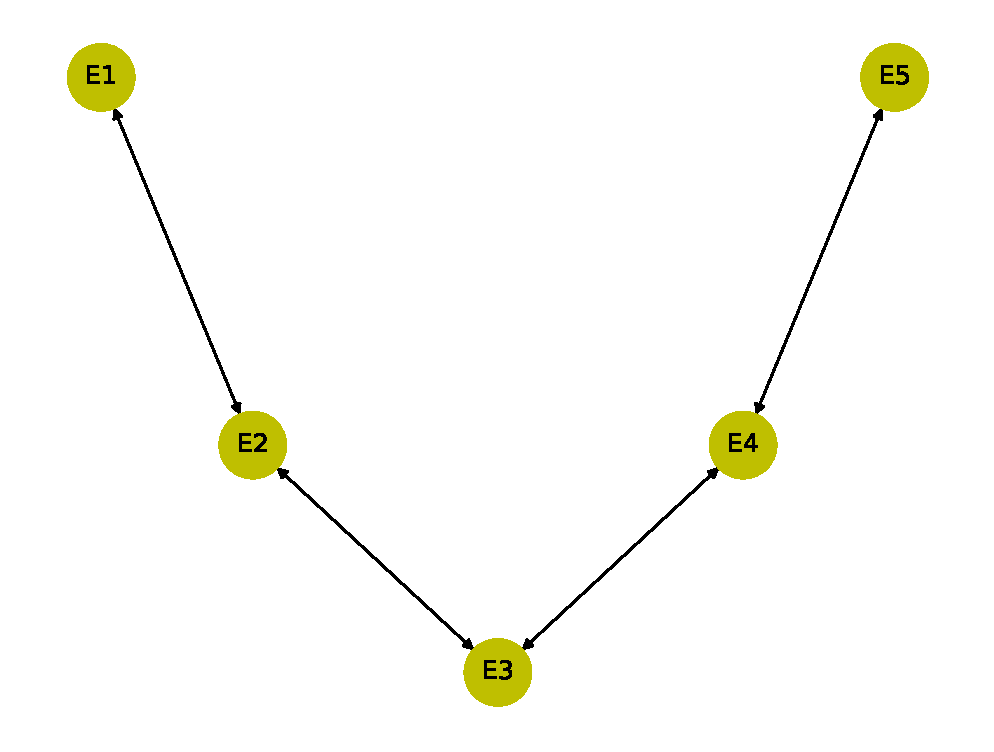
\includegraphics[scale=0.4]{MDC}
\captionof{figure}{Algoritmo espectral en multigrafo dirigido cíclico}

\end{center}

\section{Algoritmo de acomodo Fruchterman-Reingold}

La idea de este algoritmo de acomodo es considerar una fuerza entre dos nodos cualesquiera, en este algoritmo los nodos están representados por anillos de acero y los arcos son resortes entre ellos. La idea básica es minimizar la energía del sistema moviendo los nodos y cambiando las fuerzas entre ellos. En este algoritmo, la suma de los vectores de fuerza determina en que dirección se debe mover un nodo \cite{k}.\newpage

El código en python es:

\lstinputlisting[language=Python]{multigrafo_dirigido_aciclico.py}

\begin{center}

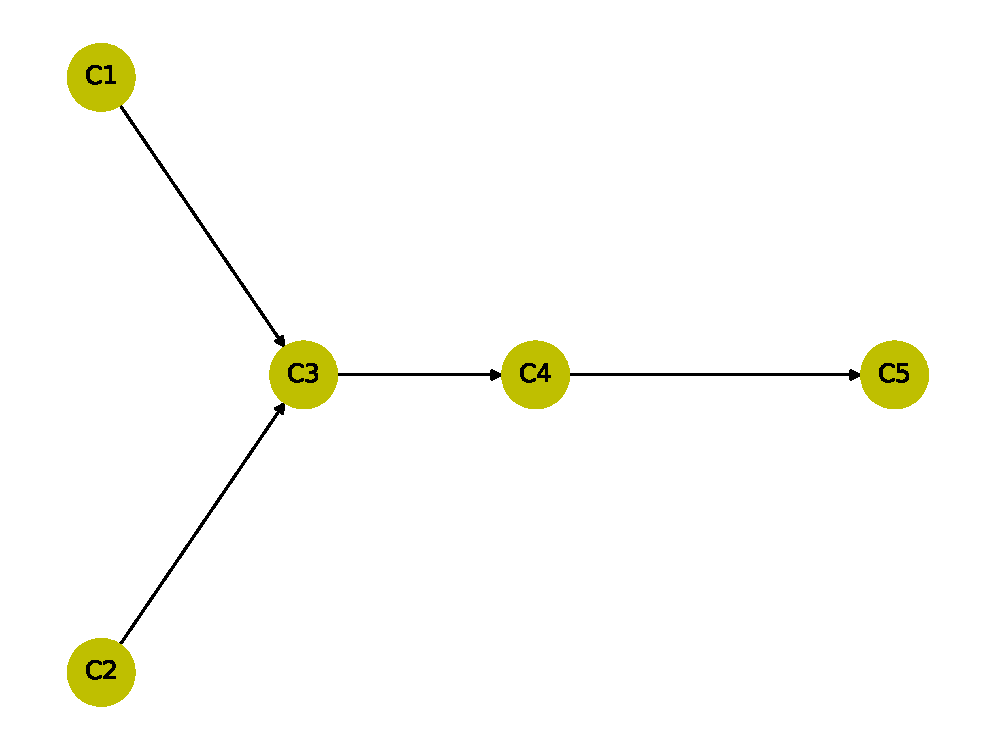
\includegraphics[scale=0.4]{MDA}
\captionof{figure}{Algoritmo fruchterman-reingold en multigrafo dirigido acíclico}

\end{center}

\section{Algoritmo de acomodo ForceAtlas2}

Es un algoritmo contínuo que permite manipular el grafo mientras se está renderizando. Cuenta con una velocidad de convergencia adaptativa única que permite que la mayoría de los grafos converjan de manera más eficiente. Propone ajustes resumidos, enfocados en qué impacto tiene la forma del grafo (escalado, gravedad,...) \cite{l}.\newpage

El código en python es el siguiente:

\lstinputlisting[language=Python]{multigrafo_no_dirigido_aciclico.py}

\begin{center}

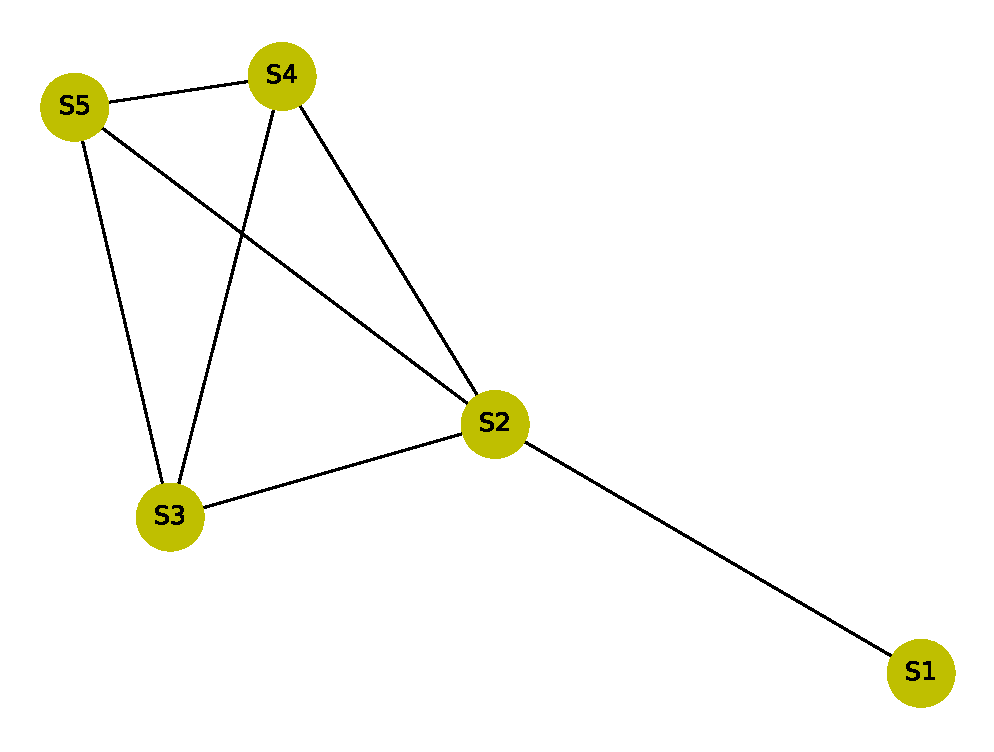
\includegraphics[scale=0.5]{MNDA}
\captionof{figure}{Algoritmo ForceAtlas2 en multigrafo no dirigido acíclico}

\end{center}

\section{Algoritmo de acomodo resorte}

El código en python se muestra a continuación:

\lstinputlisting[language=Python]{grafo_simple_dirigido_ciclico.py}

\begin{center}

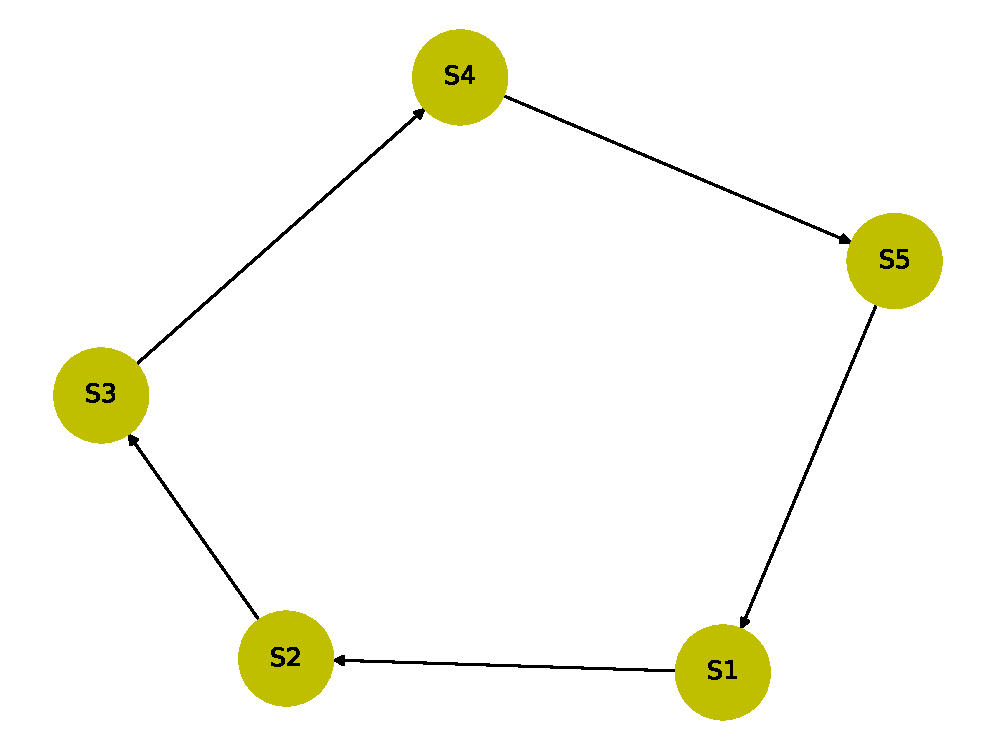
\includegraphics[scale=0.5]{GDC}
\captionof{figure}{Algoritmo resorte en grafo dirigido cíclico}

\end{center}

\section{Algoritmo de acomodo circular}

El código en python es:

\lstinputlisting[language=Python]{multigrafo_dirigido_reflexivo.py}

\begin{center}

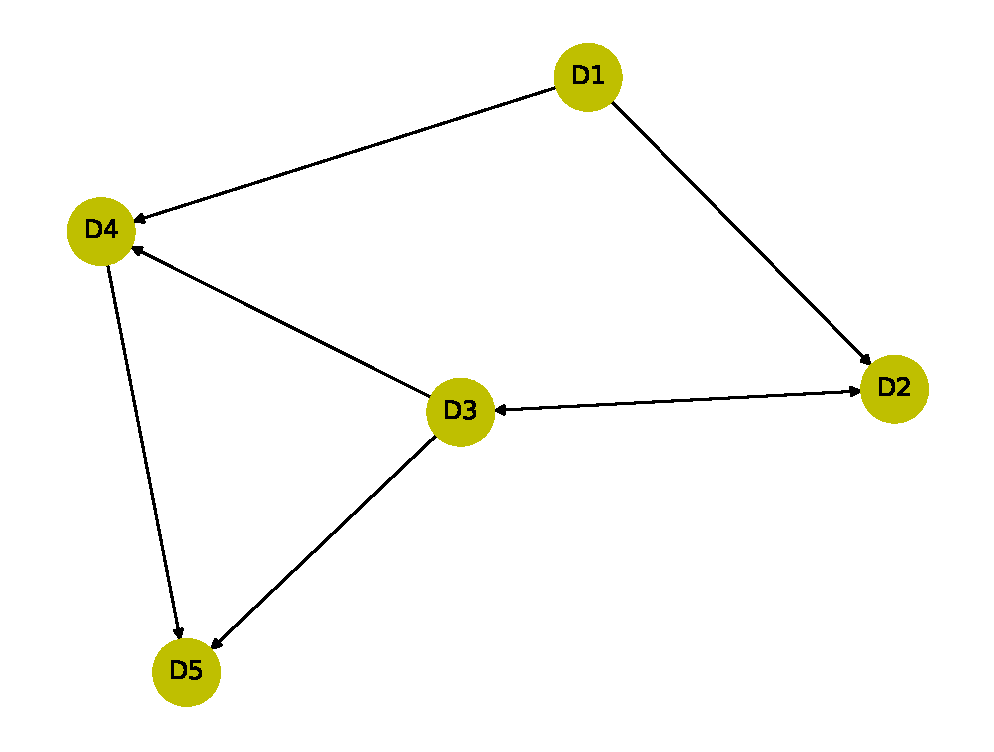
\includegraphics[scale=0.5]{MDR}
\captionof{figure}{Algoritmo circular en multigrafo dirigido reflexivo}

\end{center}

 

\bibliography{Referencias}

\bibliographystyle{plainnat}

\end{document}